\documentclass[]{article}
\usepackage{graphicx}
\usepackage{float}
\usepackage{caption}
\usepackage{amsmath}
\usepackage{amssymb}
\usepackage{bm}


%\newcommand{\deriv}[3][]{% \deriv[<order>]{<func>}{<var>}
%	\ensuremath{\frac{\partial^{#1} {#2}}{\partial {#3}^{#1}}}}

\newcommand{\derivop}[1]{% \deriv{<func>}{<var>}
	\ensuremath{\frac{\partial}{\partial {#1}}}}

\newcommand{\deriv}[2]{% \deriv{<func>}{<var>}
	\ensuremath{\frac{\partial {#1}}{\partial {#2}}}}

\newcommand{\slayer}[3]{ % scalar element of layer variable/matrix
	\ensuremath{{#1}^{(#2)}_{#3}}}

\newcommand{\vlayer}[2]{ % vector/matrix layer variable
	\ensuremath{{#1}^{(#2)}}}

\newcommand{\reals}[1]{ % vector/matrix layer variable
	\ensuremath{\in \mathbb{R}^{#1}}}

%opening
\title{Problem Set 2, Problem 2}
\author{Kireet}

\begin{document}

\maketitle

\begin{abstract}
This doc contains the derivations needed to complete the coding of the feed forward neural net problem.
\end{abstract}

\newpage
\tableofcontents
\newpage

\section{Introduction}
To run back prop, we need to calculate a bunch of derivatives with respect to the cost function. It's easiest to do the math element wise and then figure out the vectorization afterwards.

\begin{figure}[H]
\centering
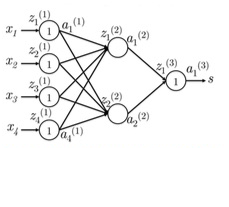
\includegraphics[width=0.7\textwidth]{neural-net}
\vspace{-7em}
\caption{A typical neural network}
\label{fig:neural-net}
\end{figure}
The above figure shows a sample 3 layer neural network with typical notation. The leftmost layer is the "input" layer, it simply receives input values $x_1$ to $x_4$ and does not do any transformation. The middle or "hidden" layer combines the input signals and the final layer again combine the hidden layer output. The hidden and output layer nodes may define non linear transformations such as the sigmoid or tanh functions. Also not pictured are linear weighting factors on each of edges of the graph. 
\paragraph{}

\marginpar{\centering
	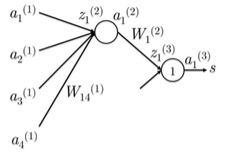
\includegraphics[width=\marginparwidth]{node}%
	\captionsetup{justification=raggedright,font={scriptsize,sf}}
	\captionof{figure}{Zoomed in view of a node in the network} }

Values related to nodes are identified by their layer and position within the layer. The input to each node is identified by $z$ and the output by $a$. Note if the node does no transformation, these values are identical. Using our standard notation, $n^{(l)}_j$ is node $j$ in layer $l$, $z^{(l)}_j$ is the input to node to that node, and $a^{(l)}_j$ is the output of the same node. The input layer is a special case, $x_j$, $z^{(1)}_j$, and $a^{(1)}_j$ all refer to the same value. The aforementioned weights between each node are identified by 3 coordinates, the input layer, the output node, and the input node. E.g. $W^{(l)}_{ij}$ refers to the weight between $n^{(l)}_j$ and $n^{(l+1)}_i$. Take note that the subscript coordinates may appear "backward" in the sense that they flow right to left in the figures. This is for mathmatical convenience.

If the subscripts are not included, then the variable refers to the vectorized representation of all values of the layer. E.g. $z^{(2)}$, $a^{(2)}$ and $W^{(2)}$ refer to all of the inputs, outputs, and weights for layer 2, respectively.

\section{Setup}
The problem states we are given a 3 layer network, the same general architecture as in Figure 1. However, we have 150 inputs at the input layer, 100 hidden nodes, and 5 output nodes. The hidden layer uses the tanh function, and the output layer uses softmax. The problem set also uses different notation:
\begin{itemize}
	\item The inputs are referred to as $L$ or $L_i$ instead of $\vec{x}$ or $x_j$. The assignment uses $x$ to actually refer to a one hot vector identifying a particular word in the vocabulary. We'll instead use $w$ for this purpose.
	\item The first weights matrix is referred to as $W$ instead of $W^{(1)}$.
	\item The second weights matrix is referred to as $U$ and is transposed. So $U^T$ is our $W^{(2)}$.
	\item Each layer has a bias input, $b^{(2)}$ and $b^{(3)}$. This is not pictured in the figures above but is standard practice. The assignment set uses 1 and 2 as the indices into layer 2 and 3 (the assignment refers to this architectures as a 2 layer network).
	\item The final output is referred to by $\hat{y}$ instead of $a^{(3)}$. We'll use $\hat{y}$ at times for convenience.
\end{itemize}
	
We will use our standard notation instead of the problem set notation. Thus:

$$w \in \mathbb{R}^{|V|} \quad \vec{x},z^{(1)},a^{(1)} \in \mathbb{R}^{150} \quad W^{(1)} \in \mathbb{R}^{100\times150} $$
$$z^{(2)},a^{(2)},b^{(2)} \in \mathbb{R}^{100} \quad W^{(2)} \in \mathbb{R}^{5\times100}$$
$$z^{(3)},a^{(3)},b^{(3)} \in \mathbb{R}^5$$
\newline

The softmax function is given as:
$$\rho(x_i) = \frac{e^{x_i}}{\sum_{j=1}^k e^{x_j}}$$
The tanh function is given as: 
$$\tau(x) =\frac{e^x - e^{-x}}{e^x + e^{-x}} = 2\sigma(2x) - 1$$

where $\sigma()$ is the sigmoid function:
$$\sigma(x) = \frac{1}{1 + e^{-x}}$$

The derivative of the tanh function can be written as a function of itself or of the sigmoid:
$$ \tau'(x) = 1 - \tau(x)^2 = 4\sigma(2x)(1-\sigma(2x))$$

Our cost function is the cross entropy loss function:
$$J(\theta) = - \sum_{k=1}^{5} y_k log(\hat{y_k})$$
where $y$ is the one hot vector identifying the correct output class.

We are asked to compute The partial derivative of $J$ with respect to $W^{(2)}$, $b^{(3)}$, $W^{(1)}$, $b^{(2)}$, and $\vec{x}$.

\section{Cross Entropy Loss/Softmax Derivative}
First we need to compute the derivative of the loss function with respect to the softmax function input, here $z^{(3)}$. It's convenient to combine these as the final result is quite simple:
$$J(\theta) = - \sum_{k=1}^{5} y_k log(\hat{y_k})$$
for a given correct class i:
$$J(\theta) = - log(\hat{y_i})$$
$$J(\theta)= - log( \frac{exp(z^{(3)}_i)} {\sum_{j=1}^5 exp(z^{(3)}_j)} )$$
$$J(\theta)= -z^{(3)}_i + log({\sum_{j=1}^5 exp(z^{(3)}_j)})$$
$$\frac{\partial{J}}{\partial{z^{(3)}_t}} = -\frac{\partial{z^{(3)}_i}}{\partial{z^{(3)}_t}} + \frac{1}{\sum_{j=1}^5 exp(z^{(3)}_j)}exp(z^{(3)}_t)$$
$$ = -\frac{\partial{z^{(3)}_i}}{\partial{z^{(3)}_t}} + \rho(z^{(3)}_t)$$
We can see the first expression will be $-1$ when $i$ = $t$, and zero otherwise. Combined with the facts that the output $\hat y_t$ is also $\rho(z^{(3)}_t)$ and $y$ is the one hot vector with a one for the correct class and zero otherwise, we can rewrite this derivative in vectorized form as a function of the feed forward output:

\begin{equation} \label{eq:d3}
\delta^{(3)} \triangleq \frac{\partial{J}}{\partial{z^{(3)}}} = \hat y - y 
\end{equation}

We define this as the "error" at layer 3 and refer to it as $\delta^{(3)}$. In general, the error at a particular layer will be the partial derivative of the cost function with respect to the input value of that layer. 

\section{Layer 3 Bias}

$$ \deriv{J}{\vlayer{b}{3}} = \deriv{J}{\vlayer{z}{3}} \cdot \deriv{\vlayer{z}{3}}{\vlayer{b}{3}} \in \mathbb{R}^5$$

The first term we know from equation \ref{eq:1} to be $\delta^{(3)}$. We need to calculate the last partial and vectorize it to complete the derivation. Note the dimensions, since $b^{(3)} \reals{5}$, the cost function derivative with respect to\vlayer{b}{3} should be as well. An important observation is that the $j^{th}$ bias only affects the $j^{th}$ output node. Thus we can simplify this to a simpler element wise derivative:

$$ \deriv{\vlayer{z}{3}}{\slayer{b}{3}{i}} = \deriv{\slayer{z}{3}{i}}{\slayer{b}{3}{i}} = \derivop{\slayer{b}{3}{i}} \left(\sum_{j=1}^{100} \slayer{W}{2}{ij}\slayer{a}{2}{j} + \slayer{b}{3}{i} \right) $$
$$ = 1 $$
Thus $ \deriv{\vlayer{z}{3}}{\vlayer{b}{3}} = \vec{1}$ which leads to

\begin{equation} \label{eq:b3}
\nabla_{\vlayer{b}{3}} = \vlayer{\delta}{3}
\end{equation}

\section{Layer 2 Weights}
This derivation is similar to the layer 3 bias derivation, but just a little bit more complex:

$$ \deriv{J}{\vlayer{W}{2}} = \deriv{J}{\vlayer{z}{3}} \cdot \deriv{\vlayer{z}{3}}{\vlayer{W}{2}} \in \mathbb{R}^{5\times100}$$

The key thing to note in this derivation is\slayer{W}{2}{ij} only affects\slayer{z}{3}{i} and thus\slayer{a}{3}{i}. Therefore:

$$ \deriv{\vlayer{z}{3}}{\slayer{W}{2}{ij}} = \deriv{\slayer{z}{3}{i}}{\slayer{W}{2}{ij}} = \derivop{\slayer{W}{2}{ij}} \left(\sum_{k=1}^{100} \slayer{W}{2}{ik}\slayer{a}{2}{k} + \slayer{b}{3}{i} \right)$$
$$ = \slayer{a}{2}{j}$$

Combining things, we have:
$$ \deriv{J}{\slayer{W}{2}{ij}} = \slayer{\delta}{3}{i} \cdot \slayer{a}{2}{j}$$

In matrix form this looks like
\[
\nabla_{\vlayer{W}{2}} = 
\begin{bmatrix}
\slayer{\delta}{3}{1}\slayer{a}{2}{1}       & \slayer{\delta}{3}{1}\slayer{a}{2}{2} & \slayer{\delta}{3}{1}\slayer{a}{2}{3} & \dots & \slayer{\delta}{3}{1}\slayer{a}{2}{100} \\
\slayer{\delta}{3}{2}\slayer{a}{2}{1}       & \slayer{\delta}{3}{2}\slayer{a}{2}{2} & \slayer{\delta}{3}{2}\slayer{a}{2}{3} & \dots & \slayer{\delta}{3}{2}\slayer{a}{2}{100} \\
\vdots	& \vdots	&\vdots	&\ddots	& \vdots \\
\slayer{\delta}{3}{5}\slayer{a}{2}{1}       & \slayer{\delta}{3}{5}\slayer{a}{2}{2} & \slayer{\delta}{3}{5}\slayer{a}{2}{3} & \dots & \slayer{\delta}{3}{5}\slayer{a}{2}{100} \\
\end{bmatrix}
\]

\begin{equation}\label{eq:W2}
\nabla_{\vlayer{W}{2}} = \vlayer{\delta}{3} (\vlayer{a}{2})^T
\end{equation}

We can double check dimensions:
$$\nabla_{\vlayer{W}{2}}\reals{5\times100},\quad \vlayer{\delta}{3}\reals{5},\quad\vlayer{a}{2}\reals{100}$$
$$\vlayer{\delta}{3} (\vlayer{a}{2})^T \Rightarrow [5\times1] * [1\times100] \reals{5\times100}$$

\section{Layer 1 Weights}
The Layer 1 weights derivation is similar to the Layer 2 derivation, but with an additional layer involved. Similar to the previous derivation, we use the fact that\slayer{W}{1}{ij} only affects\slayer{z}{2}{i}:

$$\deriv{J}{\slayer{W}{1}{ij}} = \deriv{J}{\vlayer{z}{2}} \cdot \deriv{\vlayer{z}{2}}{\slayer{W}{1}{ij}} $$
$$ = \sum_{k} \deriv{J}{\slayer{z}{2}{k}} \cdot \deriv{\slayer{z}{2}{k}}{\slayer{W}{1}{ij}}$$
$$ = \deriv{J}{\slayer{z}{2}{i}} \cdot \deriv{\slayer{z}{2}{i}}{\slayer{W}{1}{ij}}$$

First we derive the first term. Note that\slayer{z}{2}{i} impacts all of layer 3, so we can't use any simplifying assumption here.
$$\deriv{J}{\slayer{z}{2}{i}} = \deriv{J}{\slayer{a}{2}{i}} \cdot \tau'(\slayer{z}{2}{i})$$
$$ = \tau'(\slayer{z}{2}{i}) \sum_{k} \deriv{J}{\slayer{z}{3}{k}} \cdot \deriv{\slayer{z}{3}{k}}{\slayer{a}{2}{i}}$$
$$ = \tau'(\slayer{z}{2}{i}) \sum_{k} \slayer{\delta}{3}{k} \cdot \deriv{\slayer{z}{3}{k}}{\slayer{a}{2}{i}}$$
$$= \tau'(\slayer{z}{2}{i}) \sum_{k} \slayer{\delta}{3}{k} \cdot \\
\deriv{}{\slayer{a}{2}{i}}\left( \sum_{l} \slayer{W}{2}{kl}\slayer{a}{2}{k} +\slayer{b}{3}{k} \right)$$
$$ \slayer{\delta}{2}{i} \triangleq \deriv{J}{\slayer{z}{2}{i}} = \tau'(\slayer{z}{2}{i}) \sum_{k} \slayer{\delta}{3}{k} \cdot \slayer{W}{2}{ki}$$

Note that while the form of\slayer{\delta}{2}{j} differs from\slayer{\delta}{3}{i}, their meanings are similar. Namely, the derivative of the cost function with respect to the input to the layer. Now the second term:
$$\deriv{\slayer{z}{2}{i}}{\slayer{W}{1}{ij}} = \deriv{}{\slayer{W}{1}{ij}}\left(\sum_k \slayer{W}{1}{ik}x_k + \slayer{b}{2}{i} \right) $$
$$ = x_j $$

Combining these we have:
$$\deriv{J}{\slayer{W}{1}{ij}} = \slayer{\delta}{2}{i} \cdot x_j$$
Notice this is the same form as the layer 2 derivations, the derivative is some back-propagated error at the output layer multiplied by the incoming value at the input layer! It's instructive to think about the components of which \vlayer{\delta}{2} is composed: $\tau'(\vlayer{z}{2})$, \vlayer{W}{2}, and \vlayer{\delta}{3} which is itself composed of $\rho'(\vlayer{z}{3})$ and the cross entropy loss function. So we can see that all the "downstream" operations play a part in the back-propagating the error "upstream".

To vectorize operations, we can first compute \vlayer{\delta}{2}:
\[
\vlayer{\delta}{2} = 
\begin{bmatrix}
\tau'(\slayer{z}{2}{1}) \cdot (\slayer{\delta}{3}{1}\slayer{W}{2}{11} + \slayer{\delta}{3}{2}\slayer{W}{2}{21} + \slayer{\delta}{3}{3}\slayer{W}{2}{31} + ... ) \\
\tau'(\slayer{z}{2}{2}) \cdot (\slayer{\delta}{3}{1}\slayer{W}{2}{12} + \slayer{\delta}{3}{2}\slayer{W}{2}{22} + \slayer{\delta}{3}{2}\slayer{W}{2}{32} + ... ) \\
\vdots 
\end{bmatrix}
\]

\begin{equation}\label{eq:d2}
	\vlayer{\delta}{2} = \tau'(\vlayer{z}{2}) \circ \left((\vlayer{W}{2})^T\vlayer{\delta}{3}\right)
\end{equation}
We can again verify dimensions:
$$\vlayer{\delta}{2}\reals{100},(\vlayer{W}{2})^T\reals{100\times5},\vlayer{\delta}{3}\reals{5}\Rightarrow(\vlayer{W}{2})^T\vlayer{\delta}{3}\reals{100\times1}$$
\vlayer{\delta}{2}\reals{100\times1} and the element wise multiplication of 2 vectors requires their dimensions to be the same and produces a vector of the same dimensions, so \vlayer{\delta}{1}\reals{100\times1} which is correct -- there should be an error signal value for each hidden layer node.

Using this vector, we can vectorize the \vlayer{W}{1} calculation:
\[
\nabla_{\vlayer{W}{1}} = 
\begin{bmatrix}
\slayer{\delta}{2}{1}x_1       & \slayer{\delta}{2}{1}x_2 & \slayer{\delta}{2}{1}x_3 & \dots & \slayer{\delta}{2}{1}x_{150} \\
\slayer{\delta}{2}{2}x_1       & \slayer{\delta}{2}{2}x_2 & \slayer{\delta}{2}{2}x_3 & \dots & \slayer{\delta}{2}{2}x_{150} \\
\vdots	& \vdots	&\vdots	&\ddots	& \vdots \\
\slayer{\delta}{2}{100}x_1       & \slayer{\delta}{2}{100}x_2 & \slayer{\delta}{100}{5}x_3 & \dots & \slayer{\delta}{2}{100}x_{150} \\
\end{bmatrix}
\]

\begin{equation}\label{eq:W1}
	\nabla_{\vlayer{W}{1}} = \vlayer{\delta}{2}(\vec{x})^T
\end{equation}

Again let's verify dimensions to ensure the weights derivative matrix dimensions match those of the weights matrix:
$$\vlayer{\delta}{2}\reals{100},(\vec{x})^T\reals{1\times150}\Rightarrow\nabla_\vlayer{W}{1}\reals{100\times150}$$
These weight matrix derivatives / error vector calculation patterns generalize for any number hidden layers. See the lecture notes for more details.

\section{Layer 2 Bias}
The layer 2 bias derivation becomes trival now that we have the error vector\vlayer{\delta}{2}:
$$\deriv{J}{\slayer{b}{2}{i}} = \deriv{J}{\slayer{z}{2}{i}} \cdot \deriv{\slayer{z}{2}{i}}{\slayer{b}{2}{i}}$$
$$ = \slayer{\delta}{2}{i} \cdot \deriv{}{\slayer{b}{2}{i}}\sum_k \slayer{W}{1}{ik}x_k + \slayer{b}{2}{i} = \slayer{\delta}{2}{i}$$

\begin{equation}\label{eq:b2}
	\nabla_{\vlayer{b}{2}} = \vlayer{\delta}{2}
\end{equation}

\section{ Input ($\vec{x}$)}
The input derivation follows a similar pattern to the previous derivations. We can reuse previously computed expressions to simplify the work. Note that each $x_j$ impacts all of the hidden node layers:

$$\deriv{J}{x_j} = \sum_i\deriv{J}{\slayer{z}{2}{i}} \cdot \deriv{\slayer{z}{2}{i}}{x_j}$$
$$ = \sum_i \slayer{\delta}{2}{i} \cdot \deriv{}{x_j} \left( \sum_k \slayer{W}{1}{ik}x_k + \slayer{b}{2}{i} \right)$$
$$ = \sum_i \slayer{\delta}{2}{i} \cdot \slayer{W}{1}{ij}$$

Now we can vectorize:
\[
\nabla_{\vec{x}} = 
\begin{bmatrix}
\slayer{\delta}{2}{1}\slayer{W}{1}{11} + \slayer{\delta}{2}{2}\slayer{W}{1}{21} + \slayer{\delta}{2}{3}\slayer{W}{1}{31} + ...  \\
\slayer{\delta}{2}{1}\slayer{W}{1}{12} + \slayer{\delta}{2}{2}\slayer{W}{1}{22} + \slayer{\delta}{2}{2}\slayer{W}{1}{32} + ...  \\
\vdots 
\end{bmatrix}
\]

\begin{equation}\label{eq:x}
	\nabla_{\vec{x}} = (\vlayer{W}{1})^T\vlayer{\delta}{2}	
\end{equation}

Again, let's check dimensions
$$(\vlayer{W}{1})^T\reals{150\times100}, \vlayer{\delta}{2}\reals{100} \Rightarrow \nabla_{\vec{x}}\reals{150}$$
This form is very similar to the\vlayer{\delta}{2} calculation, the difference being there is no non-linear transformation at the input, so we simply have a no-op instead of the $\tau'$ element-wise product.

\section{Regularization}
Part (b) of the assignment asks us to extend the above derivations when using the regularization:
$$J_{full}(\theta) = J(\theta) + J_{reg}(\theta)$$
where:
$$J_{reg}(\theta) = \frac{\lambda}{2}\left[ \sum_{i,j} \slayer{W}{2}{ij} + \sum_{k,l} \slayer{W}{1}{kl} \right]$$

We can immediately see that this change will only affect $\nabla_{\vlayer{W}{2}}$ and $\nabla_{\vlayer{W}{1}}$ as derivatives with respect to other terms will be zero, e.g. 

$$\deriv{J_{full}(\theta)}{\vlayer{b}{2}} = \deriv{J(\theta)}{\vlayer{b}{2}}  + \deriv{J_{reg}(\theta)}{\vlayer{b}{2}}$$
$$ = \deriv{J(\theta)}{\vlayer{b}{2}} + \deriv{}{\vlayer{b}{2}}\left(\frac{\lambda}{2}\left[ \sum_{i,j} \slayer{W}{2}{ij} + \sum_{k,l} \slayer{W}{1}{kl} \right]\right)$$
$$ = \deriv{J(\theta)}{\vlayer{b}{2}} = \vlayer{\delta}{2}$$

We can also see from the above steps that the previous derivations can be left unchanged, we simply need to add the regularization derivative. Starting with the layer 2 weights:
$$\deriv{J_{reg}}{\slayer{W}{2}{ij}} = \deriv{}{\slayer{W}{2}{ij}}\left(\frac{\lambda}{2}\left[ \sum_{i,j} \slayer{W}{2}{ij} + \sum_{k,l} \slayer{W}{1}{kl} \right]\right)$$
$$ = \lambda\slayer{W}{2}{ij}$$

Thus $\nabla_{\vlayer{W}{2}}J_{reg} = \lambda\vlayer{W}{2}$ and by identical steps $\nabla_{\vlayer{W}{1}}J_{reg} = \lambda\vlayer{W}{1}$. Thus we can extend equation \ref{eq:W2}:

$$\nabla_{\vlayer{W}{2}}J_{full} = \nabla_{\vlayer{W}{2}}J + \nabla_{\vlayer{W}{2}}J_{reg}$$
\begin{equation}
\nabla_{\vlayer{W}{2}}J_{full} = \vlayer{\delta}{3} (\vlayer{a}{2})^T + \lambda\vlayer{W}{2}
\end{equation}

and equation \ref{eq:W1}:

$$\nabla_{\vlayer{W}{1}}J_{full} = \nabla_{\vlayer{W}{1}}J + \nabla_{\vlayer{W}{1}}J_{reg}$$
\begin{equation}
\nabla_{\vlayer{W}{1}}J_{full} = \vlayer{\delta}{2}(\vec{x})^T + \lambda\vlayer{W}{1}
\end{equation}
Again, we could verify dimensions, but as we previously verified the $\nabla_{\vlayer{W}{\cdot}}$ are the same as their source matrices and matrix addition is element-wise, this would be trivial.
\end{document}
